\chapter{Design og Implementering}\label{ch:Design}
Systemmet Bargainbarter er designet ud fra de krav og analyser der er beskrevet i de ovenstående sektioner. Da web applikation er lavet i ASP.Net MVC beskrives i denne sektion de forskellige dele af MVC'en, hvor der beskrives: controllere, views og Modellen. 


\section{Controllere}
Der er en overordnet rollefordeling af controllernes ansvar: 

\section{Ansvarsbeskrivelse for controllers}

\subsection{Home}
Denne controller er ansvarlig for at vise de generelle ting for hjemmesiden. Dette vil sige hovedsiden, kontakt og en About section.  

Actions
\begin{itemize}
	\item Index
	Denne action returnere et view indeholdene alle barterads i databasen. 
	\item About
	Returnere det view der hedder about med information om den BargainBarter generelt.
	\item Contact
	Action der returnere et view med contact info omkring BB.
\end{itemize}


\subsection{BarterAd}
Denne controller er overodnet ansvarlig for, at brugeren kan oprette og opdatere Barteradds annoncer på hjemmesiden. Sammenfattet: CRUD operationerne på BarterAds.

Actions:
\begin{itemize}
	\item Index er siden, hvor den pågældende bruger får vist alle BarterAds og der en knap, der directer brugeren til MakeAd-actionen.
	\item MakeAd - er siden, hvor brugeren kan oprette en annonce. Det vil sige, at brugeren kan indtaste Annoncenavn, kategori, beskrivelse og uploade et billed til en annonce. I bunden
	\item EditAd - er siden, hvor brugeren kan opdatere en af sine bytteannoncer.
	\item 
	\item
\end{itemize}

\subsection{ShowBarterAds}
Denne controller er ansvarlig for at vise BarterAds fra databasen.

Actions 
\begin{itemize}
	\item Index skal vise alle BarterAds i omvendt kronologisk rækkefølge ift. alfabetisk rækkefølge. Der skal være mulighed for at brugeren kan vælge en kategori, der directer til ShowCategori-actionen.
	\item ShowCategory skal vise alle BarterAds, der er i den valgte kategori.
	\item EditAd - returnere siden, hvor brugeren kan opdatere en af sine bytteannoncer.
	\item 
	\item
\end{itemize}


\subsection{Search}
Search-controlleren er ansvarlig for søgning i annoncerne. 

Actions 
\begin{itemize}
	\item Index(bedre navn) skal tage en tekststreng og søge i annoncerne efter match og vise en side med de matchene annoncer.
\end{itemize}

\subsection{UserProfile}
Denne controller har til ansvar at styre ansvar omkring brugerprofiler. Dette er bl.a. at vise brugerprofiler og rette i brugerprofiler.

\begin{itemize}
	\item Index Redirector blot til forsiden. Dennegiver ikke mening, da der som regel skal være et brugerId for at vide hvilken brugerprofil det drejer sig om
	\item Edit (GET) hvis brugerprofilen er den samme som den bruger man tilgår siden med, får man lov at rette i profilen, ellers returneres blot et view hvor man kan se brugerprofilen
	\item EDIT (POST) De rettede oplysninger i brugerprofilen skrives ned i databasen. Brugerprofilen bliver herefter vist.
	\item ShowUserProfile sørger for at trække data udfra databasen og sende et pænt View til siden der viser de oplysninger en brugerprofil indeholder. Hvis profilen er den samme som den bruger der tilgår den, får brugeren mulighed for at rette i oplysninger vha. en redigerknap.
\end{itemize}



\subsection{Generelle controller funktioner}\label{sc:GenerelControl}
\section{Generel controller-funktionalitet}


Generelt er der anvendt forskellige standardmetoder igennem mange af controllerne. Til data acces kalder alle controllere igennem et Unit of Work pattern, som beskrives i sektion \ref{sc:RepositoryPattern}. Til at finde den aktuelle bruger i systemet bruges HttpContext hvor brugeren findes på ID. Controllerne holder selv styr på at kalde fejl hvis de bliver kaldt med ugyldige parametre. Da dette er et meget ensartet mønster igennnem alle controllers eksemplificeres dette blot ved en enkelt controller.

\subsection{Eksemplificering af controller-funktionalitet}
Denne sektion omhandler funktionaliteten af en controller, og hvordan den fungerer. Dette er eksemplificeret igennem User storien: Opret en bytteannonce, og tager udgangspunkt i controllerens action til oprettelse af bytteannoncer.
Som det kan ses på figur \ref{fig:SDOpretAnnonceFuld} bliver actionen kaldt fra viewet. Viewet viser kun denne mulighed hvis brugeren er autentificeret, hvilket viewet, selv holder styr på. Når UI elementet bliver trykker, kalder det et Http request og serveren returnere et view til oprettelsen af BarterAds. Viewet indeholder en række forms hvor informationen om barterads kan indsættes. Denne gruppe af forms gives som parametre til aktionen når brugeren submitter. Under dette submit laver clienten et http POST til serveren, der kalder Create barterad actionen. Actionen i controlleren læser billedet brugeren har uploadet ind i et bytearray, og laver et thumbnail ud fra billedet. Igennem Httpcontext findes den aktuelle bruger, og igennem Unit of Work, gemmes annoncen i databasen på brugeren. Selve actionen returnerer et redirect til aktionen ManageAds i BarteradsControlleren. 

\begin{figure}[H]
	\centering
	\includegraphics
	[width=150mm]{figures/SDOpretAnnonceFuld.PDF}
	\caption{Sekvensdiagram for, hvordan barterAds bliver oprettet}
	\label{fig:SDOpretAnnonceFuld}
\end{figure}   

Denne beskrivelse er sigende for mange af de interaktioner der foregår på bargainbarter webstedet. De essentielle actions er kaldt igennem UI elementer der laver enten GET eller POST funktioner. Dernæst findes noget data igennem unit of work klassen der evt. behandles, hvorefter  der returneres et nyt view.


\section{Modellen}

Den endelige model (med undtagelse af den genererede indentitymodel) kan ses på figur. \ref{Manglende }. Denne model genererer databasen, ved hjælp af det tidligere beskrevede EF. Modellen er lavet ud fra domæneanalysen og implementationen af modellen tilgås af controllerne til at hente data.

\section{Data fra Database}
Når data fra databasen skal læses, overskrives eller slettes bliver Repository-pattern og UnitOfWork benyttet - mere information omkring disse kan findes i \ref{sc:RepositoryPattern}. I dette afsnit bliver det beskrevet, hvordan implementering af de forskellige CRUD-operationer på databasen er lavet. 
Da Unit Of Work og Repository-Pattern er blevet benyttet, betyder det, at al tilgang til databasen er stortset ens. Da databasen kun tilgås af UnitOfWork og GenericRepository.
Den ens tilgang til databasen betyder, at når data skal hentes i databasen skal der først oprettes et GenericRepository af den benyttede type (f.eks. UserRepository eller BarterAdRepository). 
Dette genericRepository benyttes som et håndtag til databasen, når der skal hentes data.

Over de følgende sider fremlægges sekvensdiagrammerne for, hvordan CRUD-operationerne er blevet udført for en barterad. Dette er et generelt eksempel og viser, hvordan database-trasaktionerne udføres.

\subsection{Create}
Et sekvensdiagram, for hvordan for eksempel en barterad oprettes og skrives i databasen ved brug af både UnitOfWork og GenericRepository, kan ses på figur \ref{fig:UOFSaveBarterAd}

\begin{figure}[H]
	\centering
	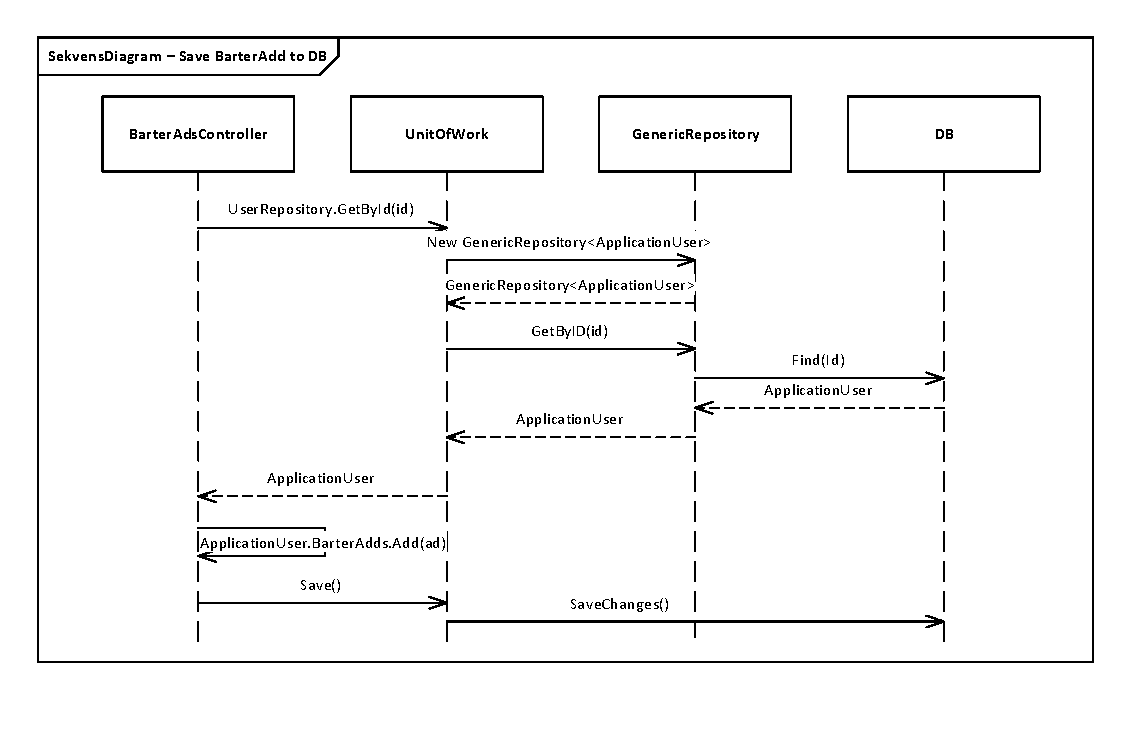
\includegraphics
	[width=150mm]{figures/SDUOFSaveBarterAd.PDF}
	\caption{Sekvensdiagram for, hvordan en barterAd bliver oprettet og gemt i DB}
	\label{fig:UOFSaveBarterAd}
\end{figure}
På sekvensdiagrammet figur \ref{fig:UOFSaveBarterAd} ses det, hvordan controlleren kalder over i unitofwork, der opretter et nyt genericrepository. Dette genericrepository gemmer barteraden i databasen.  


\subsection{Read} 
Et sekvensdiagram, for hvordan for eksempel en barterad findes og læses fra databasen ved brug af både UnitOfWork og GenericRepository, kan ses på figur \ref{fig:UOFFindBarterAd}

\begin{figure}[H]
	\centering
	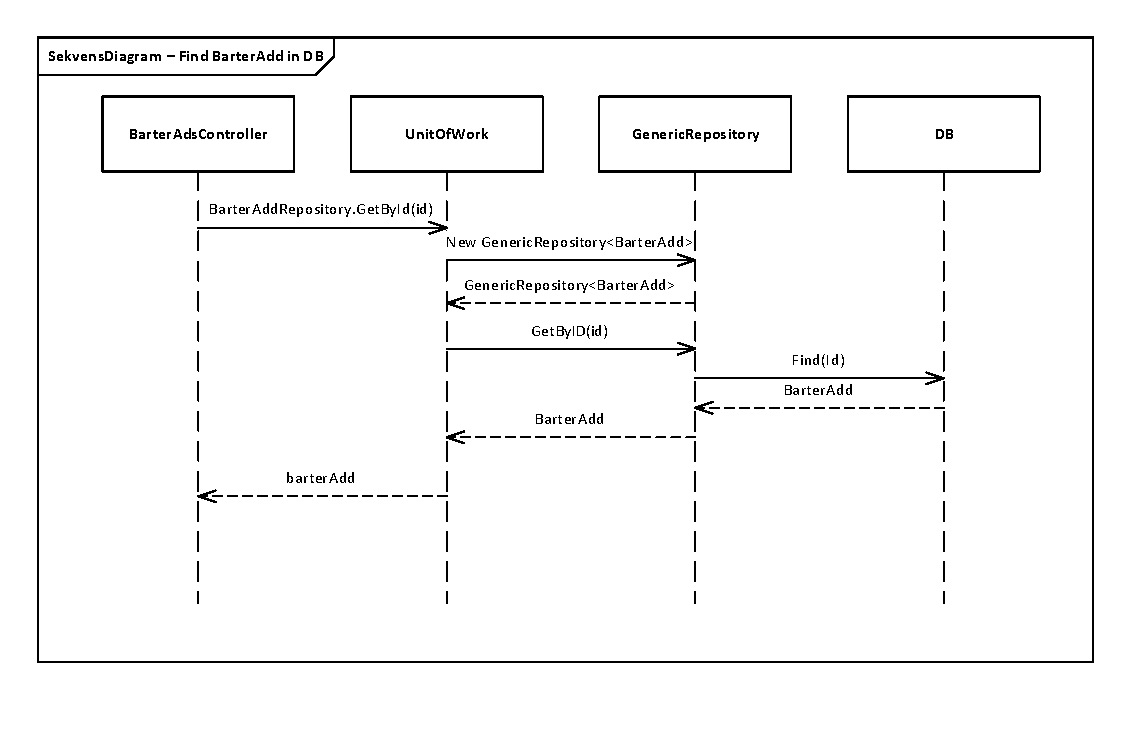
\includegraphics
	[width=150mm]{figures/SDUOFFindBarterAd.PDF}
	\caption{Sekvensdiagram for, hvordan en barterAd bliver fundet i DB}
	\label{fig:UOFFindBarterAd}
\end{figure}
På sekvensdiagrammet figur \ref{fig:UOFFindBarterAd} ses det, hvordan controlleren kalder over i unitofwork, der opretter et nyt genericrepository. Dette genericrepository finder barteraden i databasen.  


\subsection{Update}
Et sekvensdiagram, for hvordan for eksempel en barterad findes og opdateres i databasen ved brug af både UnitOfWork og GenericRepository, kan ses på figur \ref{fig:UOFUpdateBarterAd}
\begin{figure}[H]
	\centering
	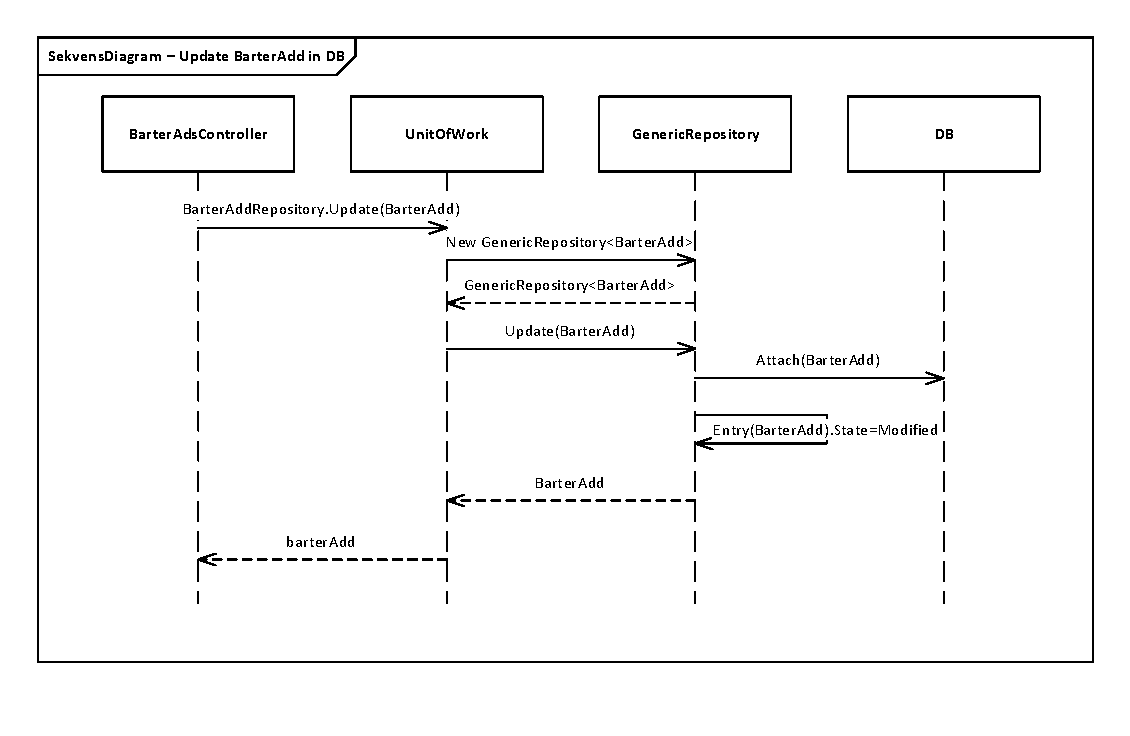
\includegraphics
	[width=150mm]{figures/SDUOFUpdateBarterAd.PDF}
	\caption{Sekvensdiagram for, hvordan en barterAd bliver opdateret i DB}
	\label{fig:UOFUpdateBarterAd}
\end{figure}
På sekvensdiagrammet figur \ref{fig:UOFUpdateBarterAd} ses det, hvordan controlleren kalder over i unitofwork, der opretter et nyt genericrepository. Dette genericrepository opdatere barteraden i databasen. 


\subsection{Delete}
Et sekvensdiagram, for hvordan for eksempel en barterad findes og slettes i databasen ved brug af både UnitOfWork og GenericRepository, kan ses på figur \ref{fig:UOFDeleteBarterAd}.
\begin{figure}[H]
	\centering
	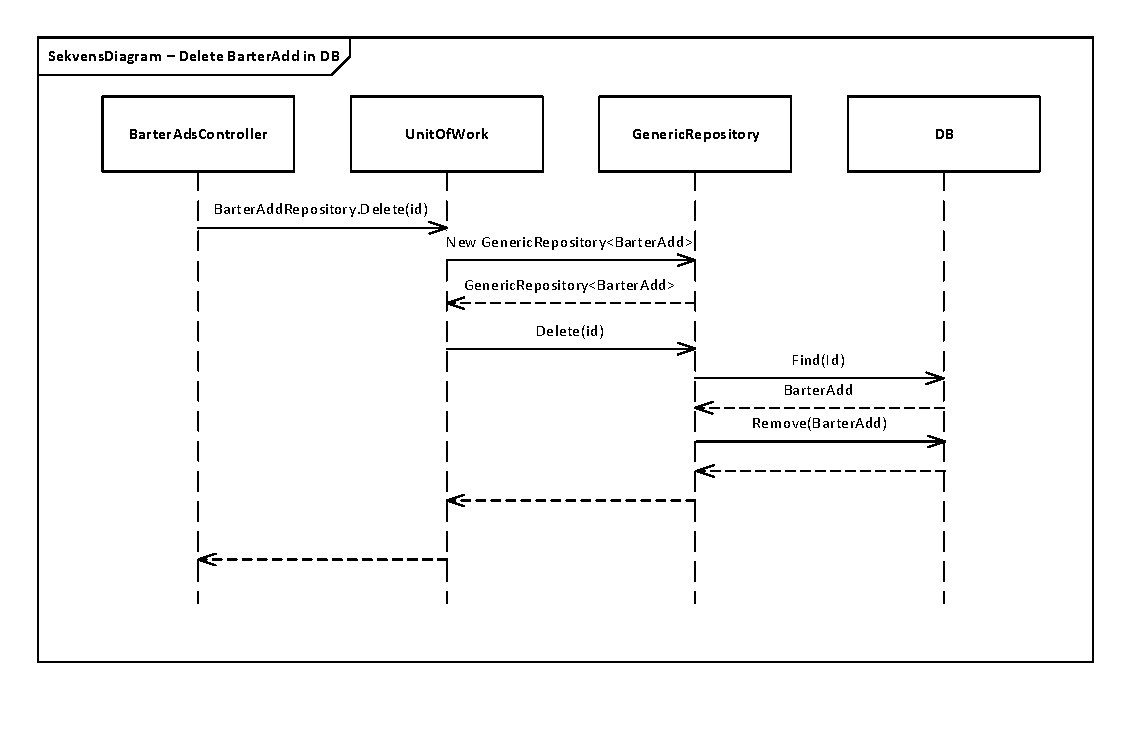
\includegraphics
	[width=145mm]{figures/SDUOFDeleteBarterAd.PDF}
	\caption{Sekvensdiagram for, hvordan en barterAd bliver slettet i DB}
	\label{fig:UOFDeleteBarterAd}
\end{figure}
På sekvensdiagrammet figur \ref{fig:UOFDeleteBarterAd} ses det, hvordan controlleren kalder over i unitofwork, der opretter et nyt genericrepository. Dette genericrepository sletter barteraden i databasen. 
